\section{Ergebnis}

Die in dieser Arbeit erbrachte Lösung ermöglicht die Überwachung der in Kapitel \ref{elemente} genannten Elemente.
% die Umsetzung der Aufgabenstellung  liefert das Produkt
%das aus der Aufgabenstellung resultierende Ausgabe beinhaltet folgende Ausgabe.
Das Ergebnis lässt sich im Webinterface von Nagios betrachten, siehe Abbildung \ref{nweb}.

%\begin{itemize}
%\item Vllt. Übersicht wie was überwacht wird
%\item Screenshots von Nagios
%\item Exportierfähigkeit, was muss alles auf dem Live-Nagios Server gemacht werden
%\end{itemize}

\begin{figure}[ht]
	\centering
	  \fbox{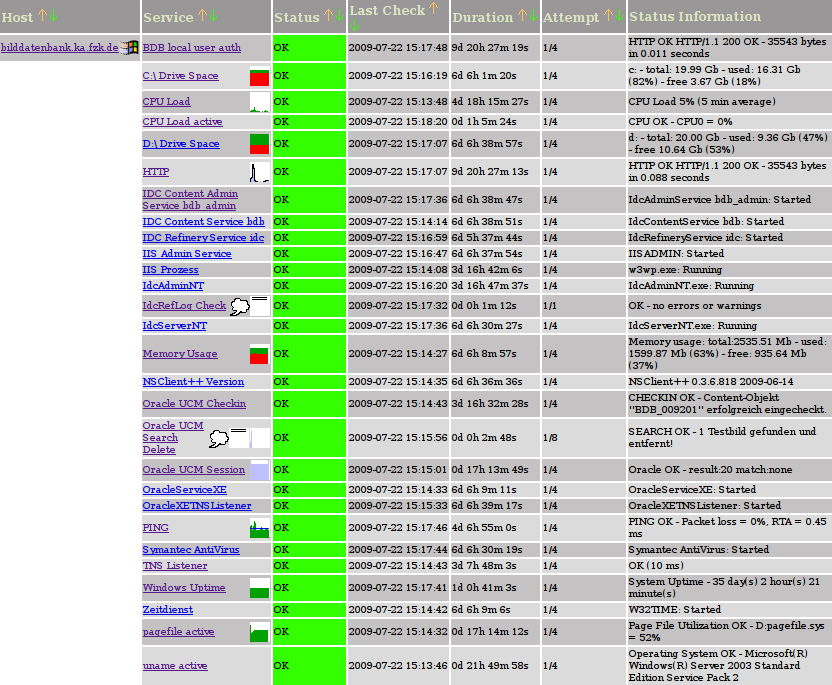
\includegraphics[width=0.93\textwidth]{bilder/demo.png}}
		\caption{Webinterface von Nagios}
		\label{nweb}
\end{figure}

Die einzelnen Elemente der Überwachung lassen sich mit Ausnahme der Benutzersimulation durch Konfiguration von bereits vorhandenen Nagios-Plugins überprüfen.
Bei dieser Konfiguration müssen die bereits im Kapitel \ref{monitor} erörterten Gesichtspunkte wie Netzwerkabhängigkeiten, -belastung und sichherheitstechnische Aspekte bedacht werden.
Gerade bei der Verwendung von Benutzerinformationen zur Authentifizierung ist es notwendig zu überprüfen, ob die Informationen als Klartext oder verschlüsselt übertragen werden.\\

Die durch die einzelnen Plugins gesammelten Informationen lassen sich zusätzlich im Detail aufrufen:

\begin{figure}[ht]
	\centering
	  \fbox{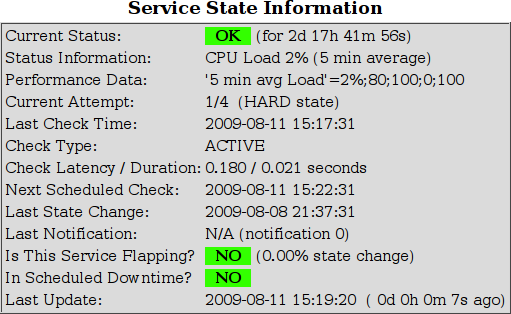
\includegraphics[width=0.8\textwidth]{bilder/cpu-load2.png}}
		\caption{Details der Prozessorauslastung}
		\label{cpuload}
\end{figure}
